\documentclass[dvipdfmx]{beamer}

\usepackage{pxjahyper}
\setlength{\parindent}{11pt}

% theme
\usefonttheme{professionalfonts}
\usetheme{Madrid}
\usecolortheme{default}
\setbeamertemplate{enumerate item}[default]
\setbeamertemplate{caption}[numbered]
\setbeamertemplate{navigation symbols}{}
\usepackage[scaled]{helvet}
\renewcommand{\sfdefault}{phv}
\renewcommand{\familydefault}{\sfdefault}
\renewcommand{\kanjifamilydefault}{\gtdefault}
\setbeamertemplate{theorems}[numbered]
\definecolor{Crimson}{HTML}{dc143c}
\setbeamercolor{alerted text}{fg=Crimson}

% graphics
\usepackage{graphicx}
\usepackage{here}
\usepackage{ulem}
% math
\usepackage{amsmath, amssymb}
\usepackage{physics}
\usepackage{mathrsfs}
\usepackage{mathtools}
%\usepackage{tikz}
%\usepackage[all]{xy}
\mathversion{bold}
\definecolor{math}{HTML}{100080}
\everymath{\color{math}}

% theoremstyle
\usepackage{amsthm}
\newtheoremstyle{break}
{\topsep}{\topsep}%
{}{}%
{\bfseries}{}%
{\newline}{}%
\theoremstyle{break}
\newtheorem{thm}{Theorem}[section]
\newtheorem{defn}[thm]{Definition}
\newtheorem{eg}[thm]{Example}
\newtheorem{cl}[thm]{Claim}
\newtheorem{cor}[thm]{Corollary}
\newtheorem{rem}[thm]{Remark}
\newtheorem{ax}[thm]{Axiom}
\newtheorem{prob}{Problem}[section]

\makeatletter
\newenvironment{pr}[1][\proofnam]{\par
\topsep6\p@\@plus6\p@ \trivlist
\item[\hskip\labelsep{\itshape #1}\@addpunct{\bfseries}]\ignorespaces
}{%
\endtrivlist
}
\newcommand{\proofnam}{\underline{Derivation.}}
\makeatother



% link

\usepackage{url}
\usepackage{hyperref} 
\usepackage{xcolor}
\usepackage{pxjahyper}
\definecolor{link}{HTML}{4b0082}
\hypersetup{
	colorlinks=true,
	citecolor=link,
	linkcolor=link,
	urlcolor=orange,
}

% my command
\newcommand{\hilb}{\mathcal{H}}
\newcommand{\R}{\mathbb{R}}
\newcommand{\C}{\mathbb{C}}
\newcommand{\Z}{\mathbb{Z}}



% title
\author[T. Tanaka]{Toshiya Tanaka}
\institute[Univ. Toyama]{University of Toyama}
%\author[田中]{田中寿弥}
%\institute[富大理物]{富山大学理学部物理学科}
\title[\textcolor{white}{プログラミング入門}]{数物系のためのPC・プログラミング入門}
%\subtitle{}
\begin{document}
\begin{frame}
		\maketitle
\end{frame}


\begin{frame}{はじめに}
		\begin{alertblock}{注意}
				\begin{itemize}
						\item 初学者向けです.
						\item 私も初学者です.
						\item 初学者のうちだからこそ,初学者がつまづきやすいところがわかるかもしれません.
				\end{itemize}
		\end{alertblock}
		\begin{block}{プログラミングが必要になる場面}
				\begin{itemize}
						\item \LaTeX によるレポート,論文執筆
						\item 数値計算
						\item 関数をプロットし,振る舞いを確認する
						\item 実験の解析
						\item 研究室,研究会のHP管理
				\end{itemize}
		\end{block}
		もちろん極めようと思えばキリがないですが,ちょっとしたプログラミングができると人生がラクになります.
\end{frame}

\section{Linux}
\begin{frame}{OS}
		大きく分けて,次の三つがあります.
		\begin{itemize}
				\item Windows
				\item Mac
				\item Linux
		\end{itemize}
		Windowsは{\sout{\textcolor{gray}{カス}}}
		プログラミングに向いていないので,Linuxをおすすめします.
\end{frame}


\section{プログラミング}
\begin{frame}{プログラミング言語}
		\begin{table}
				\centering
				\begin{tabular}{c|c}\hline
						言語 & 特徴\\\hline
						Python & \begin{tabular}{l}
								難易度は易しめ.\\
								環境構築せずとも,google colabolatryなど\\オンラインサービスがある.\\
								パッケージが豊富に存在.
								\end{tabular}\\\hline
						Haskell & 関数型言語.圏論と関連があるらしい.\\\hline
						Julia & 早い.ギリシア文字なども使える.\\\hline
				\end{tabular}
		\end{table}
\end{frame}

\begin{frame}[fragile]
		\begin{columns}
				\begin{column}{0.45\textwidth}
						\begin{block}{julia}
\begin{semiverbatim}
using SpecialFunctions
using Plots

x = 1:5
y = factorial.(x)
scatter(x, y)
plot!(x->gamma(x+1), 
    ylims=(0, 130))
savefig("gamma.png")
\end{semiverbatim}
						\end{block}
				\end{column}
				\begin{column}{0.45\textwidth}
		\begin{figure}
				\centering
				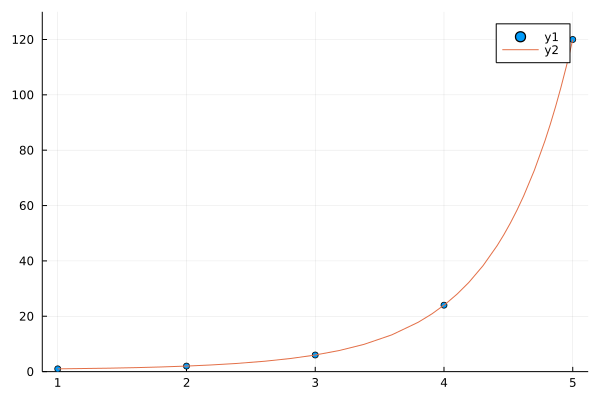
\includegraphics[width=5cm]{./plot/gamma.png}
				\caption{$n!$と$\Gamma(x+1) $}
		\end{figure}
				\end{column}
		\end{columns}
\end{frame}
\section{LaTeX}
\begin{frame}{\LaTeX}
		\begin{block}{できること}
				\begin{itemize}
						\item 美しい数式の組版
						\item スライド作成
				\end{itemize}
		\end{block}
\end{frame}
\end{document}


